\documentclass[twoside]{EPURapport}
%\usepackage{listings}
\usepackage[utf8]{inputenc}

%\renewcommand{\lstlistlistingname}{Liste des codes}
%\renewcommand{\lstlistingname}{Code}

%\addextratables{%
%	\lstlistoflistings
%}

%\swapAuthorsAndSupervisors



\usepackage[utf8]{inputenc}

\usepackage{hyperref}

\thedocument{Projet d'option web}{Évolution d'un classifieur multimédia, interactif et en ligne}{Projet d'option web - Évolution d'un classifieur multimédia, interactif et en ligne}

\grade{Département Informatique\\ 5\ieme{} année\\ 2012 - 2013}

\authors{%
	\category{Étudiants}{%
		\name{Adrien BATAILLE} \mail{adrien.bataille@etu.univ-tours.fr}
		\name{Valentin DOULCIER} \mail{valentin.doulcier@etu.univ-tours.fr}
	}
	\details{DI5 2012 - 2013}
}

\supervisors{%
	\category{Encadrants}{%
		\name{Gilles VENTURINI} \mail{gilles.venturini@univ-tours.fr}
		\name{Fabienne DALINO} \mail{fabienne.dalino@gmail.com}
	}
	\details{Université François-Rabelais, Tours}
}

\abstracts{Description en français}
{Mots clés en Français}
{Description en anglais}
{Mots clés en anglais}

\begin{document}


\chapter{Introduction}

Ce présent document est un rapport de projet se rattachant à l'option Web \& Multimédia. Il a pour but de présenter à la fois les demandes du client, mais aussi le travaille effectué ainsi que les process mis en place.
	
Notre projet s'effectue par binôme dans le cadre de notre formation en dernière année au département informatique de Polytech' TOURS.\\

Le client de notre projet est l'équipe INNOPHYT. Cette équipe fait partie de l'Université François Rabelais de Tours et est consacrée aux activités de valorisation et de recherche dans le domaine de la lutte anti-parasitaire durable. Nos encadrants de projet sont Gilles VENTURINI ainsi que Fabienne DALINO. N'ayant pas de contact avec le client, ils sont des interlocuteurs pour les aspects techniques et opérationnels.

	\section{Contexte}
	
	L'enjeu global du projet est mettre à disposition de l'équipe INNOPHYT un outil performant d'aide à la décision de reconnaissance d'insecte, et plus précisément, de savoir si une espèce est nuisible ou non.\\
	
	Anciennement, l'équipe INNOPHYT utilisait un fichier Excel qui répertoriait l'ensemble des questions à se poser pour arriver à un résultat. Ces questions étaient disposées sous une forme d'une arborescence compliquée. Ce système étant quelque peu archaïque et n'étant pas vraiment ergonomique, un premier projet collectif s'est donc inscrit dans ce sens en modernisant l'outil (Développement d'une application android). Suite à cette application, décuplant les performances et les fonctionnalités, la question du site web dédié s'est posée. En réponse, un projet web s'est donc mis en place, et à répondu partiellement à l'ensemble des besoins énoncés.\\
	
	Les futurs utilisateurs de l'application dans sa version site web sont nombreux. Ils peuvent être aussi bien des ingénieurs ou des spécialistes du domaines (biologiste de terrain, membre de l"équipe INNOPHYT...) que des utilisateurs lambda n'ayant pas de connaissances particulières (agriculteur, passionné des insectes...). A ce titre, la version web de l'application pourra s'utiliser à titre pédagogique, et pourra servir d'outils de formation et de découverte.	
	
	\section{Objectif}
	
	Notre projet s'inscrit dans la continuité d'un projet débuté l'année dernière, dans le même contexte éducatif que nous, et dont le but était de développer la structure du site.\\
	
	L'objectif est donc de fournir une application web reproduisant les spécificités de l'application android. Principalement, le but de notre projet est, à partir de la lecture d'un fichier XML représentant un arbre de décision, de permettre à l'utilisateur  de naviguer dans cet arbre dans le but de trouver l'insecte qu'il observe.\\
	
	Le site web calquera son interface ergonomique et convivial sur celle de la tablette. Ainsi, l'utilisateur jonglant entre les deux plateformes ne sera pas perdu en passant de l'une à l'autre. Nous implémenterons donc l'ensemble des fonctionnalités présentes sur la tablette, afin que l'utilisation ne soit en rien différente.

	\section{Contraintes technologiques}
	
	Dans notre cas, les termes "Contraintes Technologiques" ont pris tous leurs sens. En effet, notre projet s'inscrivant dans la suite d'un projet préalablement commencé, nous avons été obligé de réutiliser certaines librairies mises en place ainsi que certaines technologies.\\
	

	\begin{itemize}
		\item \textbf{Bootstrap} : Dans le but de poser les bases du design, la librairie Bootstrap a été choisie. Il s'agit de la bibliothèque développée et utilisée par le célèbre Twitter. En plus des feuilles de style CSS, Bootstrap comprend un certain nombre de composants intéressants comme des boutons, des menus, une barre de chargement... Il contient aussi quelques plugins JavaScript comme le Carrousel, qui ont servi à l'affichage des galeries de médias.\\
		
		\item \textbf{Shadowbox} : Cette librairie permet de lire tous types d'objets multimédias (vidéo, son, image) dans une fenêtre modale, et ainsi de profiter de toute la largeur de l'écran. Elle est toutefois très limitée dans l'interaction dynamique avec un serveur, notamment dans le cadre de chargement de formulaire.\\
		
		\item \textbf{Flash} : Pour l'affichage de la webcam, il s'agit d'un code minimaliste en Flash. En effet, cela permet de démarrer la webcam après autorisation de l'utilisateur, et d'afficher simplement à l'écran l'image filmée en temps réel.\\
		
		\item \textbf{Ajax} : Permet de rendre l'interface plus conviviale, nous avons décidé de mettre en place une architecture AJAX. Cela permet notamment de supprimer les rechargements de pages inutiles. Le problème rencontré est que tout le site a été passé en AJAX, ce qui ne facilite absolument pas la navigation (gestion des pages précédentes...).\\
		
		\item \textbf{jQuery} : Nous avons utilisé JQuery et ses fonctions spécialisées dans l'architecture AJAX pour simplifier la gestion de notre application. Aussi, certaines fonctionnalités de Jquery (à savoir Jqplot), nous ont permis de générer facilement les graphiques demandés.\\
	\end{itemize}
	
	Différents problèmes ont été rencontré avec ces contraintes, ils sont respectivement détaillés dans la parties concernant les librairies \ref{lib}.



\chapter{Architecture}

Dans cette partie, nous allons détailler les différents points sur lesquelles nous avons travaillé ainsi que les problèmes rencontrés. De plus, nous verrons toutes les librairies utilisées au sein de ce projet ainsi que des explications plus complètes sur les problèmes et avantages de celles-ci.

	\section{Le site rba-innophyt}
	
		\subsection{Login}
		
\begin{figure}[hbtp]
			\centering
			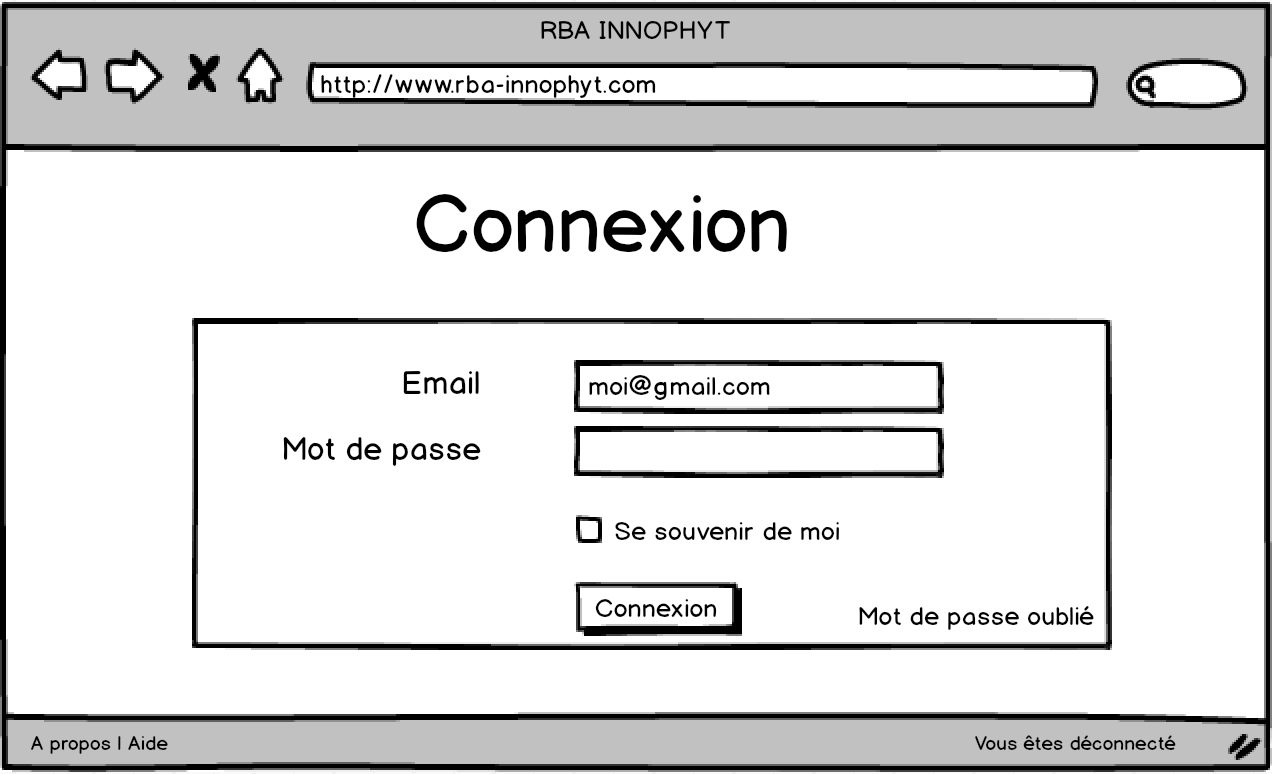
\includegraphics[scale=0.5]{images/login.png}
			\caption{Schéma de login}
		\end{figure}			
		
		
			\subsubsection{Sécurité}
			\subsubsection{Footer}
		\subsection{Menu}
		
			L'organisation du menu nous est apparu assez évidente lorsque nous avons étudié l'application tablette. En effet, nous avons choisi de reprendre la même ergonomie afin de ne pas perdre l'utilisateur lorsqu'il change de plateforme. A ce titre, nous nous sommes inspirés du menu iCloud, disposant sur 2 rangées un ensemble de blocs, chacun correspondant à une fonctionnalité élémentaire de l'application.\\
			
			\begin{figure}[hbtp]
			\centering
			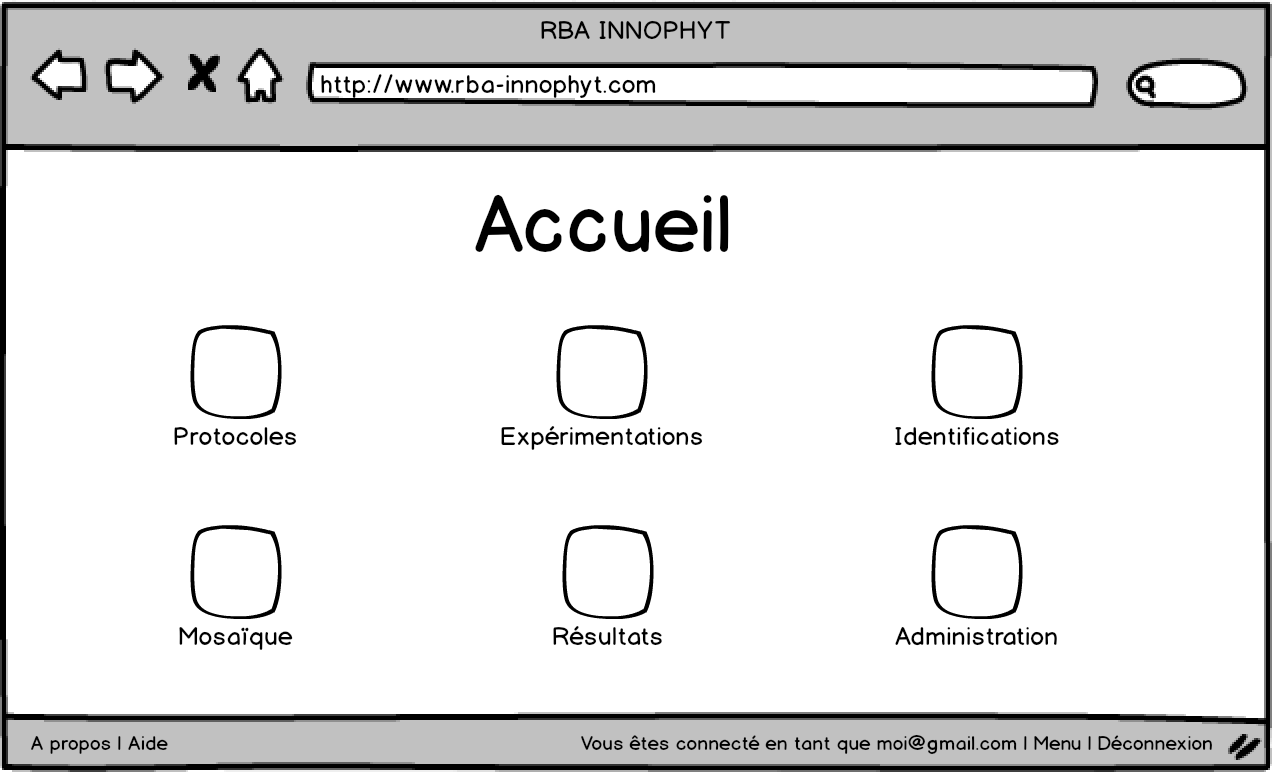
\includegraphics[scale=0.5]{images/menu.png}
			\caption{Schéma du menu}
		\end{figure}	
		
		\subsection{Campagne / Parcelle / Piège}
		
	S'inspirant du fonctionnement déjà mis en place sur la tablette, nous avons implémenté les divers écrans permettant à l'utilisateur de sélectionner sa campagne, sa parcelle ainsi que son piège.\\
	
	Nous avons toutefois choisi d'ajouter de nouvelles fonctionnalités, comme le fait de pouvoir visualiser la localisation des pièges sur une google map (classés par type), ainsi que des statistiques sur les espèces répertoriées dans les pièges. L'affichage des statistiques se fait grâce à l'utilisation de graphiques (import des librairies correspondantes, voir partie 2.3).
		
		\subsection{Arbre de décision}
		
		L'implémentation de l'affichage de l'arbre de décision étant le principal intérêt du précédent projet web, nous n'avons que très peu modifier cette partie là. Nous nous sommes contentés de rajouter quelques détails, notamment sur l'écran résultat. Celui-ci dispose maintenant des champs nécessaires à la saisie du nombre d'insecte trouvé, et nous avons renommé les libellés à la demande des clients. Aussi, nous utilisons désormais les images miniatures générées via le menu Administrateur. Le contenu des pages est alors moins lourd.
		
		\subsection{Mosaïque}

	Toujours dans l'esprit d'implémenter les mêmes fonctionnalités sur la tablette que sur le site internet, nous avons développé le module mosaïque. Ce module parse l'ensemble du fichier xml de l'arbre de question, et répertorie l'ensemble des fichiers images résultats. Une fois ces images répertoriées, nous effectuons un tri afin d'éliminer les doublons. Pour finir, nous affichons dans des carrés de taille identique les images redimensionnées, sur lesquels l'utilisateur avertis pourra cliqué afin de saisir directement une récolte.\\
	
	Les images affichées sur l'écran mosaïque sont des images retouchées quant à leurs dimensions initiales. En effet, dans un soucis de détail, les images parcourues dans le dossier média initial pèsent approximativement entre 3 et 6 Mo, ce qui est très lourd pour des images en 400x400. A ce titre, notez bien que les miniatures doivent être disponible afin d'afficher la mosaïque. Pour se faire, un administrateur doit se rendre sur l'écran d'administration, et cliquer sur générer les thumbnails. Cette opération n'est à effectuer qu'une seule fois, ainsi qu'à chaque modification du dossier média (ajout de résultats ou de branches dans l'arbre).\\
	
	L'arbre que nous avons testé contient environ 100 résultats images. Nous sommes partis du principe que l'utilisateur ne disposait pas forcément d'une connexion ultra rapide. A ce titre, nous avons utilisé une méthode qui permets de charger progressivement les résultats à l'écran. Ainsi, les images sont chargées au fur et à mesure que l'utilisateur scroll sur la page mosaïque, ce qui permets un affichage nettement plus fluide ainsi qu'une meilleur expérience utilisateur (temps de chargement quasi invisible).

		\subsection{Export}
		
	Similaire au comportement que l'on retrouve sur la tablette, nous avons implémenté une fonction d'export des données saisies par l'utilisateur. Ainsi, l'export permets de récupérer au format csv (lisible par excel par exemple) l'ensemble des données, bien formatées, que l'utilisateur a pu enregistrer au cours de ses récoltes.\\
	
	Les champs répertoriés sont identiques à ceux récupérés sur l'application tablette.\\
	
	Le fonctionnement est assez simple, il s'agit d'exécuter une requête sql permettant de récupérer, dans l'ordre désiré, les différents champs à inscrire dans le fichier csv. On y place dans un premier temps l'en-tête des colonnes, puis les données, bien séparées par le symbole ";".\\
	
	Nous avons toutefois rencontré une petite difficulté, puisque certaines notes contenant des retours à la ligne, le programme générant le csv l'interprétait comme un changement de champ. Ainsi, chaque fois qu'un retour à la ligne était détecté, on se retrouvait avec un décalage d'une case, l'export perdant ainsi tout son sens. Nous avons résolu le problème en modifiant l'interpréteur des données récupérées par la requête. Ainsi, grâce notamment à des fonctions de trim, les données se mettent désormais toujours à leur place, permettant une lecture de données intègre dans l'export csv.	
		
		
		\subsection{Administration}
		
	Le module d'administration est un bloc disponible uniquement dans la version site web de l'application. Ce bloc n'est accessible qu'aux personnes présentant les droits requis pour y accéder.\\
	
	Une des fonctionnalités de ce module est de pouvoir générer les thumbnails. Ce sont les images miniatures, permettant d'afficher de façons plus légère le contenu média de l'arbre et de la mosaïque.\\
	
	La seconde fonction principale de ce module est la gestion des utilisateurs. Chaque utilisateur est donc répertorié dans un tableau, et l'on peut alors pour chacun d'eux modifier les caractéristiques (Administrateur, login, mot de passe, plage d'adresses IP ...).
		
		\subsection{À propos}
		
	La section à propos, que l'on retrouve dans le footer, est un module que l'on retrouve également sur l'application android. Celle-ci permets de retrouver le nom des collaborateurs au projet (financeurs, auteurs, partenaires) ainsi qu'un onglet comment faire, et bibliographie. Le contenu n'a volontairement pas été ajouté, il conviendra aux administrateurs de modifier ces textes afin de mettre la description qui leur convient.\\
	
	En ce qui concerne le premier onglet, on applique toujours la même ergonomie en ce qui concerne l'affichage des informations. Chaque logo est placé dans un carré de taille similaires aux autres. L'objectif est ici de garder une cohérence à travers tout le site.	
	
	\subsection{Aide}
		
		Pour accéder à l'aide, nous avons créé un lien dans le footer. Lorsque l'on clique dessus, une pop-up s'affiche, et demande à l'utilisateur s'il souhaite envoyer un mail ou bien consulter l'aide en ligne (fichier pdf). Si le choix de l'utilisateur se porte sur le mail, le client mail par défaut s'ouvre, et on observe les champs pré-remplis. Le fichier PDF n'est quant à lui pas rédigé, il appartiendra à l'administrateur du site de rédiger une aide en ligne et de faire le lien avec la demande utilisateur.
		

	\section{Arborescence}
	
	Dès la prise en main du projet, nous avons choisis de modifier de A à Z l'arborescence de base de ce projet. En effet, celle-ci ne permettait pas d'avoir une solution propre et viable sur le terme. De ce fait nous avons regroupé les fichiers CSS et JavaScript respectivement dans les dossiers \emph{css} et \emph{js}. Toutes les images, hormis celles utilisées pour l'arbre de décision et la mosaïque sont dans le dossier \emph{images}. Enfin, les librairies qui avait chacune leur dossier ont été divisées entre plusieurs dossiers. En effet, leurs fichiers CSS et JavaScript ont été mis dans les dossiers correspondant, et les fichiers spécifiques ont été déplacé dans un dossier \emph{lib}.\\

	Ces modifications permettent une meilleure évolution du site et facilite l'ajout de module et partie. Voici plus en détail le contenu des différents dossiers.
	
	\begin{figure}[hbtp]
			\centering
			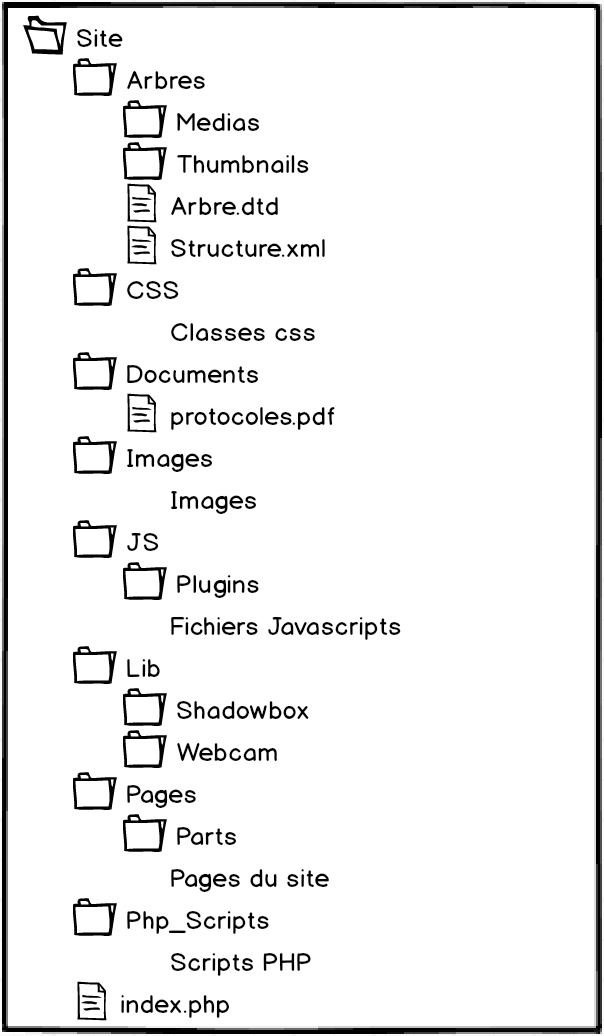
\includegraphics[scale=0.6]{images/arborescence.png}
			\caption{Schéma succin de l'arborescence}
		\end{figure}

		\subsection{arbres}
		Ce dossier contient à sa racine le fichier \emph{arbre.dtd} permettant de contrôler la structure des xml contenant les arbres de décision. Il y a aussi la présence d'un dossier \emph{medias} contenant toute les images originales de l'arbre. Quant à lui, \emph{thumbnail} contient toutes les miniatures générées et utilisées pour l'affichage de la mosaïque ou des photos galeries dans l'arbre de décision.
		
		\subsection{css}
		Ce dossier contient tous les fichiers css utilisés pour le style du site. Aussi bien pour les librairies (\emph{Bootstrap} \ref{lib:bootstrap}, \emph{jqPlot} \ref{lib:jqplot}, \emph{jQuery UI} \ref{lib:jqueryui} et \emph{Shadowbox} \ref{lib:shadowbox}) que le fichier \emph{syle.css} où est le style personnalisé du site.
		
		\subsection{documents}
		Ce dossier contient tous les fichiers annexes utilisés sur le site tel que la liste des protocoles ou le guide utilisateur de la plate-forme web.
		
		\subsection{images}
		Ce dossier contient toutes les petites images et icônes utilisées sur le site comme par exemple pour le menu, les marqueurs Google Map \ldots
		
		\subsection{js}
		Ce dossier contient tous les fichiers JavaScript utilisés dans le site. Aussi bien pour les librairies (\emph{Bootstrap} \ref{lib:bootstrap}, \emph{jQuery} \ref{lib:jquery}, \emph{jqPlot} \ref{lib:jqplot}, \emph{jQuery UI} \ref{lib:jqueryui} et \emph{Shadowbox} \ref{lib:shadowbox}) que les fichiers propres à chacune des parties du site.
		
		\subsection{lib}
		Ce dossier contient les fichiers propres aux différentes librairies utilisés dans le site comme pour la webcam et le player pour les fichiers multimédias de la pop-up shadowbox.
		
		\subsection{pages}
		Ce dossier contient les fichiers php qui correspondent respectivement aux différentes pages du sites.
		
			\subsubsection{part}
			Ce sous-dossier contient toutes les différentes sous-parties qui se retrouve dans toutes les pages comme par exemple le \emph{header}, le \emph{footer} \ldots
		
		\subsection{php\_script}
		Ce dossier contient tous les fichiers php qui sont utilisés côté serveur pour faire toutes les actions avec la base de données comme par exemple lister les campagnes ou ajouter un utilisateur.
	
	\section{Librairies}
	\label{lib}
		
		\subsection{API Google Map}
		\label{lib:map}
		Nous avons utilisé l'API Google Map afin d'afficher sur une carte les différent pièges d'une parcelle grâce à différents marqueurs. Cette API pour fonctionner nécessite une clé, mais nous avons réussis à l'utiliser sans. Au lieu d'inclure le script sous la forme \url{https://maps.googleapis.com/maps/api/js?key=GOOGLE_MAP_API_KEY&sensor=false}, nous utilisons \url{http://maps.google.com/maps/api/js?sensor=false}.
		
		\begin{figure}[hbtp]
			\centering
			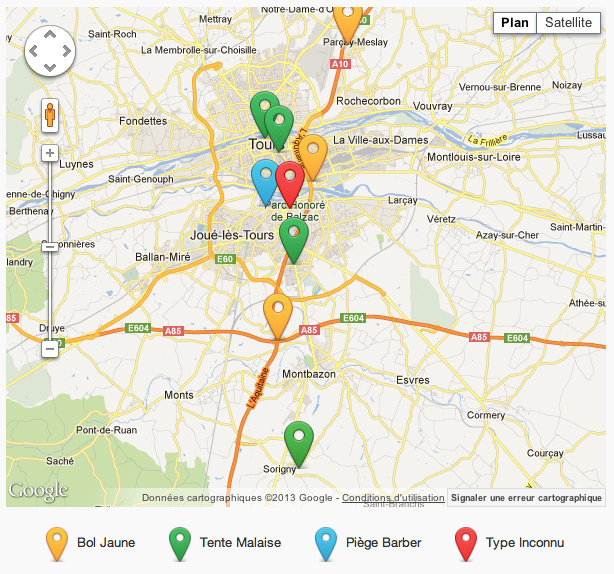
\includegraphics[scale=0.5]{images/lib-API_GoogleMap.png}
			\caption{Carte Google Map des emplacements des pièges}
		\end{figure}
		
		\subsection{jQuery}
		\label{lib:jquery}
		jQuery est une librairie JavaScript qui permet de manipuler le DOM (Document Object Model), gérer les événements, créer des effets visuels mais aussi d'effectuer des requêtes Ajax.
		
		\subsection{jQuery UI}
		\label{lib:jqueryui}
		jQuery UI est un ensemble de plugins qui permet d'avoir un certain nombre de composant graphique. Nous l'avons utilisé pour mettre en place le datepicker dans les formulaires d'ajout et de modification des campagnes, parcelles et récoltes.
		
		\begin{figure}[hbtp]
			\centering
			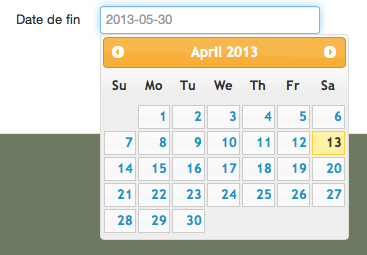
\includegraphics[scale=0.5]{images/lib-jquery_datePicker.png}
			\caption{Le date picker de jQuery UI}
		\end{figure}
	
		\subsection{jqPlot}
		\label{lib:jqplot}
		jqPlot est un plugin de traçage et de la cartographie pour jQuery. jqPlot produit des graphiques en lignes, bars et camemberts avec de nombreuses fonctionnalités. Cette librairie nous permet d'afficher les graphiques montrant la répartition des différents régimes alimentaires des récoltes d'un piège.
		
		\begin{figure}[hbtp]
			\centering
			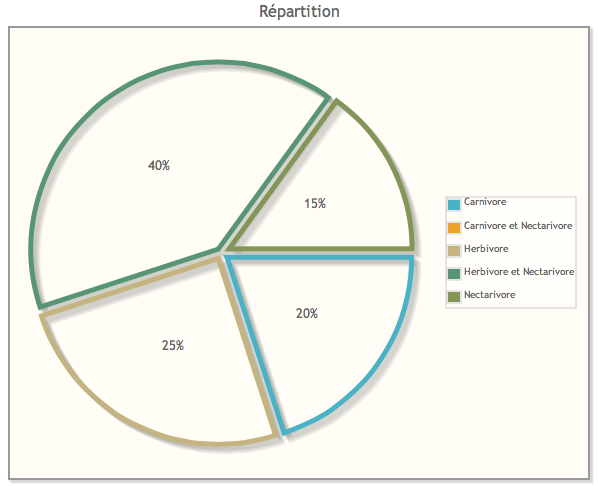
\includegraphics[scale=0.5]{images/lib-jqplot.png}
			\caption{Camenbert de répartition des insectes}
		\end{figure}
		
		
		\subsection{Bootstrap}
		\label{lib:bootstrap}
		Bootstrap est une bibliothèque développée et utilisée par Twitter. En plus des feuilles de style CSS, Bootstrap comprend un certain nombre de composants intéressants comme des boutons, des menus, une barre de chargement... Il contient aussi quelques composant JavaScript comme le Carrousel, ce dernier est utilisé pour  afficher les galeries de médias.\\
		
		Le problème majeur que nous avons rencontré avec cette librairie et que la version utilisée à plus d'un an. Nous avons donc essayé de la mettre à jour, notamment les fichier CSS afin d'avoir les derniers effets qui nous n'avons pas. Or, le groupe qui a fait la première version de l'arbre de décision que nous avons intégré à notre projet à tout simplement modifié directement les fichiers CSS de Bootstrap. De ce fait, il nous est impossible de les remplacer par les nouveaux sans casser tout le style actuel du site.
		
		\subsection{Shadowbox}
		\label{lib:shadowbox}
		ShadowBox permet de lire tous type d'objets multimédias (vidéo, son, image) et afficher du HTML dans une fenêtre modale, et aussi profiter de toute la largeur de l'écran.
		
		\begin{figure}[hbtp]
			\centering
			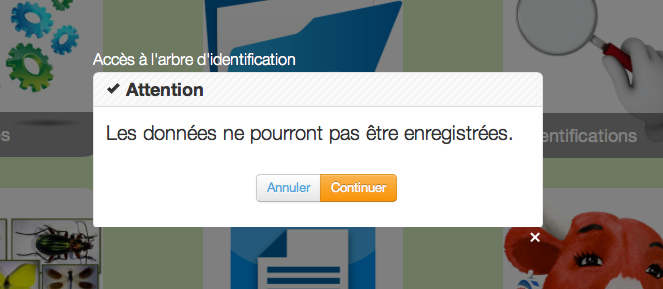
\includegraphics[scale=0.5]{images/lib-shadowbox.png}
			\caption{Utilisation de Shadowbox}
		\end{figure}
		
		\subsection{Webcam}
		\label{lib:webcam}
		Un code minimaliste en Flash est inclut dans le site, il nous permet de démarrer la webcam après autorisation de l'utilisateur, et d'afficher à l'écran l'image filmée.
		
		\begin{figure}[hbtp]
			\centering
			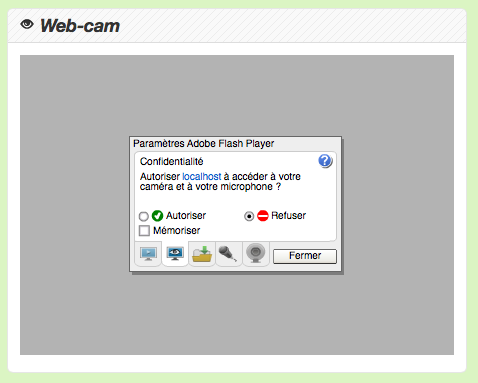
\includegraphics[scale=0.5]{images/lib-webcam.png}
			\caption{Utilisation de la Webcam}
		\end{figure}
	
	\section{Technologies}
	\label{tec}
	
		\subsection{Ajax}
		\label{tec:ajax}
		Ajax (Asynchronous JavaScript and XML) est utilisé pour récupérer et échanger de façon asynchrone au chargement de la page du contenu sur le serveur. Cette technologie est utilisée pour l'arbre d'identification avec le chargement des questions.
		
		\subsection{Web Storage}
		\label{tec:storage}
		Web Storage est une solution adaptée aux besoins actuels de stockage de données variées, dans le navigateur. C'est aussi une technique plus puissante que les cookies, qui sont limités en taille (quelques Ko contre plusieurs Mo pour Web Storage) et qui engendrent un trafic HTTP supplémentaire pour chaque requête.\\
		
		Web Storage met à disposition deux interfaces nommées \emph{sessionStorage} et \emph{localStorage} dont la seule différence concerne la persistance des données. Ces dernières ne sont plus véhiculées sur le réseau HTTP et elles sont facilement accessibles (lecture, modifications et suppression) pour la programmation en JavaScript.\\
		
		Nous utilisons le Web Storage pour stocker aussi bien l'authentification de l'utilisateur que des données diverses et variées pour le fonctionnement du site. Par exemple, lors d'une identification, la campagne, la parcelle et le piège choisis sont stocker dans le localStorage. Les différentes clés utilisées pour stocker ces informations sont dans le fichier \emph{variable.php}

\chapter{Analyse Critique}

	\section{Du projet}
	
	Dire ce qui est bien, cool dans se qu'on a fait et les points qui peuvent être améliorés
	
	\section{Améliorations}
	
	Donner les points à améliorer pour les prochains projets

\chapter{Conclusion}

Ce projet s'inscrivant dans la continuité d'un projet précédent, une des premières choses que nous avons faite a été de chercher à comprendre le fonctionnement de la version que nous avons reprise. C'est une tâche plus ardue qu'il n'y parait, dans le sens où la logique développeur peut être propre à chacun de nous. L'inconvénient principal que nous avons noté est bien sur les technologies que nous avons du reprendre, et qui selon nous n'ont pas toujours été bien choisies.\\

Toutefois, ce projet s'est avérer être très intéressant. Il nous a donné l'occasion une fois de plus de mettre en pratique nos connaissance. Le sujet du site web nous a également plu, ce qui nous a motivé pour développé un produit propre, facile à maintenir et parfaitement fonctionnel.

\annexes

\end{document}